\documentclass{report}

\usepackage{verbatim}
\usepackage[utf8]{inputenc}
\usepackage[italian]{babel}
\usepackage[table]{xcolor}
\usepackage[T1]{fontenc}
\usepackage[shortlabels]{enumitem}
\usepackage{wrapfig,hyperref,listings,amsfonts,makecell,enumerate,
            array,graphicx,plain,setspace, multicol, caption,
	        titlesec,blindtext,nameref,geometry}
%\usepackage[export]{adjustbox} 
\renewcommand{\arraystretch}{1.4}
%\setlength{\cellspacetoplimit}{4pt}
%\setlength{\cellspacebottomlimit}{4pt}

\geometry{
	paperheight = 29.7cm,
	paperwidth = 21cm,
	outer = 1.5cm,
	inner = 2.5cm,
	top = 2cm,
	bottom = 2cm
}
\singlespacing

% nessuna interruzione di pagina tra capitoli
%\renewcommand{\cleardoublepage}{}
%\renewcommand{\clearpage}{}

% redefinizione del formato del titolo del capitolo
%\titleformat{\chapter}
%	{\normalfont\Huge\bfseries}{\thechapter}{1em}{}

%------ chapter -----
\definecolor{gray75}{gray}{0.75}
\newcommand{\hsp}{\hspace{20pt}}
\titleformat{\chapter}[hang]{\normalfont\Huge\bfseries}{\thechapter\hsp\textcolor{gray75}{|}\hsp}{0pt}{\Huge\bfseries}
\titlespacing*{\chapter}{0pt}{-20pt}{40pt}

\definecolor{Gray}{gray}{0.9}

% -------- figure in multicols ----------
\newenvironment{Figure}
  {\par\medskip\noindent\minipage{\linewidth}}
  {\endminipage\par\medskip}

\begin{document}

\pagestyle{plain}
\thispagestyle{empty}

\graphicspath{{assets/figures/}}

\begin{center}
	\begin{figure}[h!]
		\centerline{
\includegraphics[width=0.6\textwidth]{Img/logo_unitn_black_center.eps}}
	\end{figure}

	\vspace{2 cm}

	\LARGE{Dipartimento di Ingegneria e Scienza dell’Informazione}

	\vspace{1 cm}

	\Large{
		Corso di Laurea in\\
		Informatica
	}

	\vspace{2 cm}
	\Large\textsc{Progetto Ingegneria del Software\\}
	\vspace{1 cm}
	\Huge\textsc{Sistema di monitoraggio ambientale\\}
	\vspace{1cm}
	\Large{D4 G19}

	\vspace{4cm}

	\Large{Anno accademico 2021/2022}
\end{center}
\tableofcontents
\chapter*{Scopo del documento}
\addcontentsline{toc}{chapter}{Scopo del documento}
Il documento presentato riporta tutte le informazioni necessarie per lo sviluppo dell'applicativo Sistema Monitoraggio Ambientale. In particolare, esso presenta tutti gli artefatti necessari per sviluppare le funzionalità dell'account di tipo Amministratore, definito nei precedenti documenti. Partendo dalla descrizione delle user stories, features ed user flow legate al ruolo di amministratore, il documento procede con la presentazione delle API necessarie per poter visualizzare, modificare ed inserire i dati dei sensori GPS utilizzati dall'applicazione. A seguire troveremo un capitolo  dove sarà possibile vedere come è stata pensata l'interfaccia utente, con l'obiettivo di essere la più semplice e chiara possibile.
Per ogni API presentata, oltre alla descrizione delle funzionalità fornite, il documento presenta la documentazione ed i casi di test correlati.


\chapter{User Stories}

Una "User Story" è una descrizione informale e generica di una caratteristica del software presentata dal punto di vista dell'utente finale.\\
Il punto focale di ogni User Story presentata nel documento viene posto sull'amministratore, ossia l'utente principale da noi selezionato per l'implementazione dell'applicazione. Esso è in grado sia di visualizzare i dati relativi al parco in termini di popolazione, dei rischi ambientali e delle descrizioni dei singoli animali, sia di gestire i sensori GPS dei singoli animali. \\
Ogni User Story viene definita con un linguaggio non tecnico, volta a fornire allo sviluppatore un'idea del chi (Who?), cosa (What?) e del perchè(Why?) si sta sviluppando una specifica funzionalità del software.
Le \textbf{User Stories} legate all'Amministratore dell'applicazione "Sistema di monitoraggio ambientale" sono riportate nella tabella seguente. Nel caso non sia presente un requisito funzionale o non funzionale, viene presentata una "X" ad indicare che non esiste tale correlazione.\\

\begin{table}[ht]
    \centering
    \begin{tabular}{|m{0.05\linewidth}|m{0.38\linewidth}|m{0.20\linewidth}|m{0.25\linewidth}|}
    \hline
        & \textbf{Descrizione User Story} & \textbf{Requisiti funzionali} & \textbf{Requisiti non funzionali} \\
        \hline
        \rowcolor{Gray}
        \textbf{US1} & Come amministratore voglio poter selezionare il parco in cui mi trovo, per vedere le informazioni di quest’ultimo & RF 2.1 &  X \\
        \hline
        \textbf{US2} & Come amministratore voglio poter visualizzare le specie di flora e fauna, per vedere le informazioni degli animali e delle piante & RF 2.1 & X \\
        \hline
        \rowcolor{Gray}
        \textbf{US3} & Come amministratore voglio poter visualizzare le statistiche del parco in termini di pericolo ambientale così da poterlo tenere sotto controllo & RF 2.3 & RNF 3.3 \\
        \hline
        \textbf{US4} & Come amministratore voglio poter visualizzare, per la specie animale selezionata, un istogramma rappresentante la sua popolazione nel tempo e una mappa delle posizioni degli animali di quella specie in tempo reale, in modo da tenerli sotto controllo & X & RNF 2.5, RNF 3.3 \\
        \hline
        \rowcolor{Gray}
        \textbf{US5} & Come amministratore, voglio essere in grado di selezionare un sensore GPS del parco per poi eliminarlo, in modo da poterlo gestire & RF 2.5 & X \\
        \hline 
        \textbf{US6} & Come amministratore, voglio essere in grado di aggiungere un sensore GPS nel parco, in modo da poterlo gestire & RF 2.5 & X \\
        \hline
        \rowcolor{Gray}
        \textbf{US7} & Come amministratore, voglio essere in grado di selezionare un sensore GPS del parco per poi visualizzarne i dati, in modo da poter ottenere informazioni sul singolo elemento & RF 2.5 & X \\
        \hline
    \end{tabular}
\end{table}
\chapter{Features}
\begin{table}[ht]
    \centering
    \begin{tabular}{|m{0.09\linewidth}|m{0.2\linewidth}|m{0.63\linewidth}|}
    \hline
        \textbf{User Story} & \textbf{Feature index} & \textbf{Feature} \\
        \hline
        \rowcolor{Gray}
        US1 & F1 & Mostrare i parchi selezionabili utilizzando una lista.\\
        \hline
        US1 & F2 & Estrarre tutti i parchi memorizzati tramite un’API locale.\\
        \hline
        \rowcolor{Gray}
        US1 & F3 & Mostrare la pagina del parco selezionato.\\
        \hline
        US2 & F4 & Mostrare le specie presenti nel parco selezionato utilizzando un elenco.\\
        \hline
        \rowcolor{Gray}
        US2 & F5 & Estrarre tutte le specie presenti nel parco tramite un’API locale.\\
        \hline
        US3 & F6 & Mostra pagina contenente le statistiche ambientali.\\
        \hline
        \rowcolor{Gray}
        US3 & F7 & Estrarre le statistiche ambientali memorizzate tramite un’API locale.\\
        \hline
        US4 & F8 & Mostrare le specie presenti nel parco selezionato utilizzando un elenco.\\
        \hline 
        \rowcolor{Gray}
        US4 & F9 & Estrarre tutte le specie presenti nel parco tramite un’API locale.\\
        \hline
        US4 & F10 & Mostrare pagina con la mappa contenente le posizioni degli animali e l’istogramma sullo storico della popolazione.\\
        \hline 
        \rowcolor{Gray}
        US4 & F11 & Estrarre tutte le posizioni dell’animale selezionato tramite un’API locale.\\
        \hline
        US4 & F12 & Estrarre lo storico dell’animale selezionato tramite un’API locale.\\
        \hline 
        \rowcolor{Gray}
        US5 & F13 & Mostrare pagina con i dati dei sensori GPS tramite un elenco.\\
        \hline
        US5 & F14 & Estrarre i dati dei sensori tramite un’API locale filtrati con il parco selezionato dall’amministratore.\\
        \hline
        \rowcolor{Gray}
        US5 & F15 & Mostrare un’area contenente i dati del sensore selezionato.\\
        \hline
        US5 & F16 & Predisporre un bottone per eliminare il sensore.\\
        \hline
        \rowcolor{Gray}
        US5 & F17 & Aggiornare il database tramite un’API locale.\\
        \hline
        US6 & F18 & Mostrare una pagina con i dati dei sensori tramite un elenco.\\
        \hline
        \rowcolor{Gray}
        US6 & F19 & Estrarre i dati dei sensori tramite un’API locale, filtrati con il parco selezionato dall’amministratore.\\
        \hline
        US6 & F20 & Predisporre un bottone per aggiungere un sensore.\\
        \hline
        \rowcolor{Gray}
        US6 & F21 & Visualizzare un form con dei campi da compilare per aggiungere un sensore.\\
        \hline 
        US6 & F22 & Memorizzare sul database i dati del nuovo sensore tramite un’API locale.\\
        \hline
        \rowcolor{Gray}
        US7 & F23 & Mostrare una pagina contenente i dati dei sensori tramite un elenco.\\
        \hline
        US7 & F24 & Estrarre i dati dei sensori tramite un’API locale filtrati con il parco selezionato dall’amministratore.\\
        \hline 
        \rowcolor{Gray}
        US7 & F25 & Visualizzare un’area contenente i dati del singolo sensore.\\
        \hline
    \end{tabular}
\end{table}
\chapter{User Flows}
\label{capitolo3}
In questa sezione vengono presentati gli User Flows correlati alla figura dell'Amministratore da noi scelta. La figura \ref{fig:userFlow} descrive lo User Flow relativo alla gestione ed ottenimento delle informazioni del parco, già introdotte nel capitolo introduttivo. In qualsiasi momento l'amministratore può gestire e visualizzare i sensori presenti nel parco e visualizzare informazioni inerenti la flora e la fauna del suddetto.

Nella figura \ref{fig:userFlow} vengono anche presentate le relazioni tra le azioni effettuate da parte dell'amministratore e le features descritte nel capitolo precedente. In aggiunta viene posta una legenda per facilitare la comprensione del diagramma sottostante.

%\newpage

\begin{figure}[ht]
    \centering
    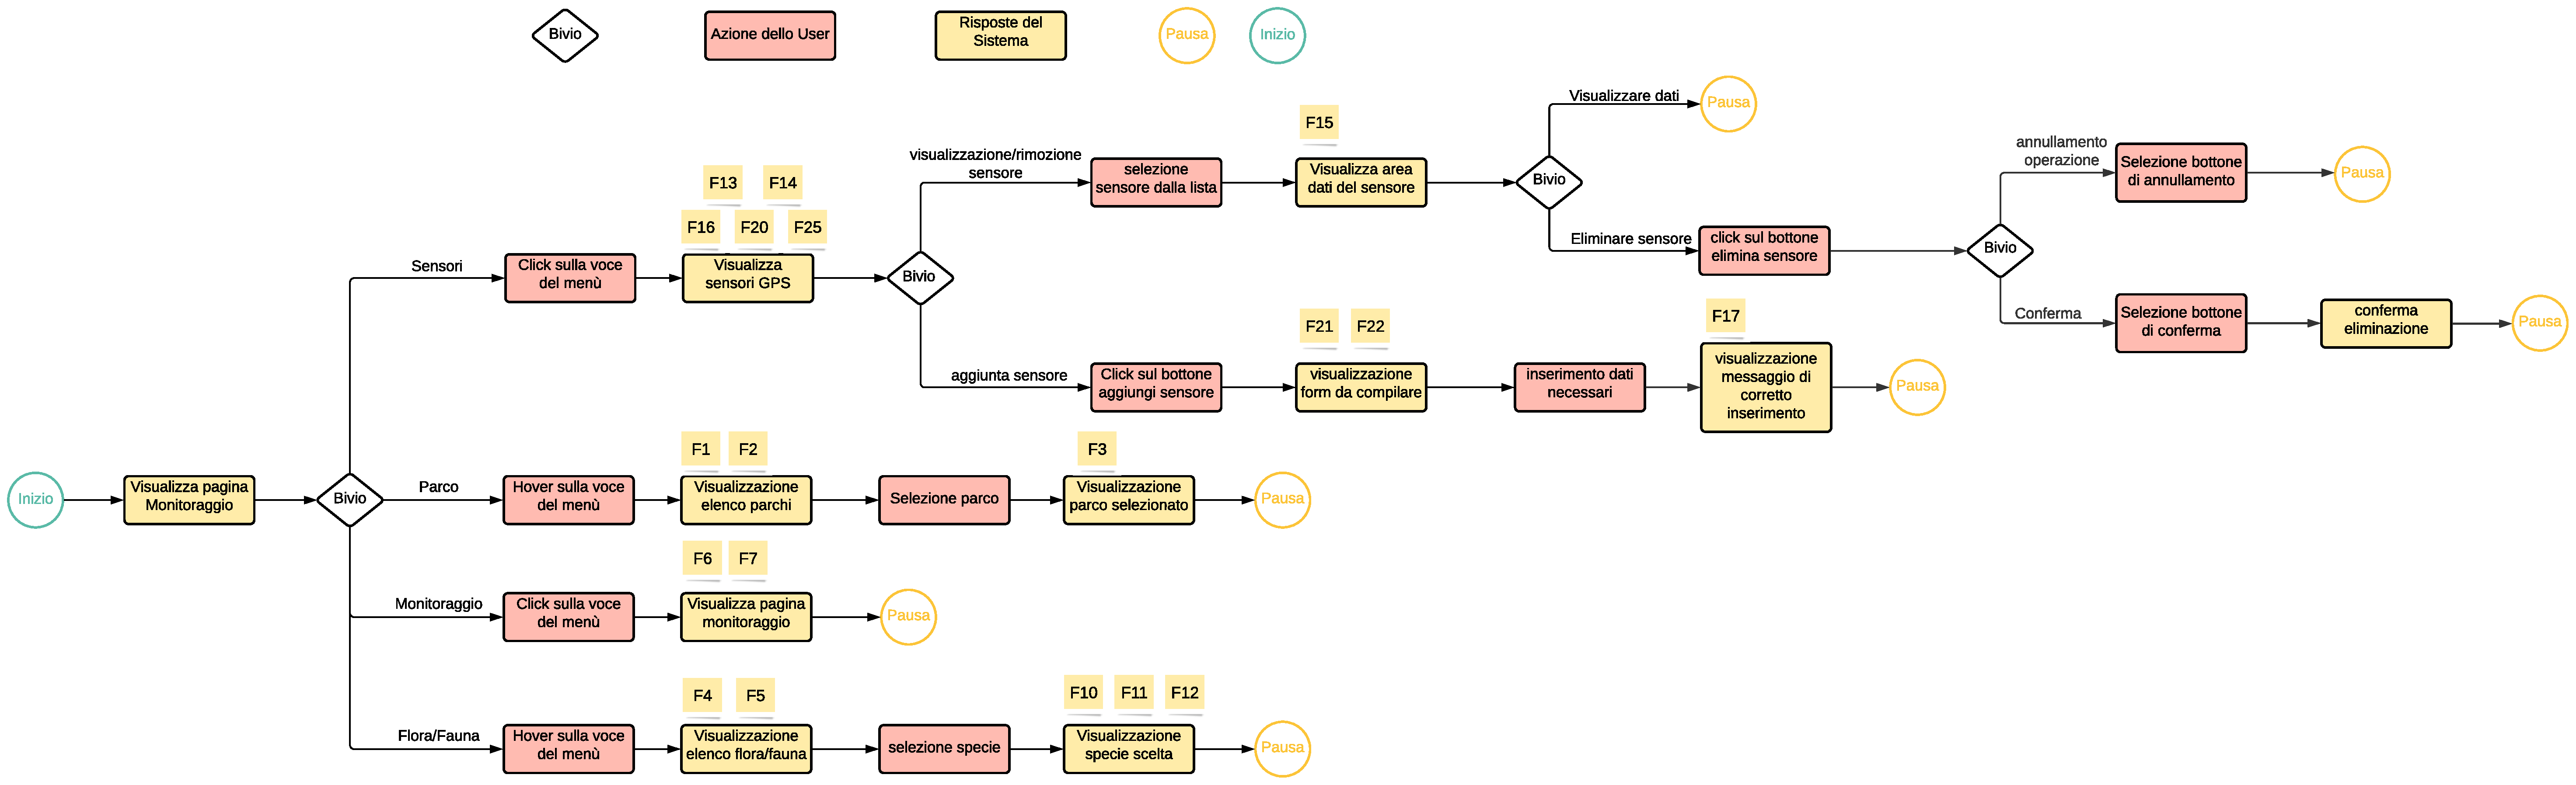
\includegraphics[scale=0.25,angle=90,origin=c]{Img/userFlow.eps}
    \caption{User flow}
    \label{fig:userFlow}
\end{figure}

\chapter{Application Implementation and \\ Documentation}

Nei capitoli precedenti sono state presentate le features che devono essere implementate per il corretto funzionamento dell'applicazione Sistema Monitoraggio Ambientale nel caso in cui dovesse essere utilizzata da un utente di tipo Amministratore.
L'applicazione è stata sviluppata con \texttt{NodeJS} e \texttt{Bootstrap}. Per la gestione dei dati abbiamo utilizzato \texttt{MongoDB}.

\section{Project Structure}

Nella figura \ref{fig:projectStructure} possiamo vedere la struttura del progetto.
Esso è composto da una cartella api per la gestione delle API locali, una cartella css che contiene un file di stile, una cartella images che contiene tutte le immagini utilizzate nel progetto, una cartella js che raggruppa tutti i file javascript e infine una cartella ui che contiene le le pagine html. In fondo si può vedere anche la pagina html principale dell'applicazione e il file README.md utilizzato da github per fornire una descrizione del progetto contenuto nella repository e come eseguirlo correttamente.

\begin{figure}[ht]
    \centering
    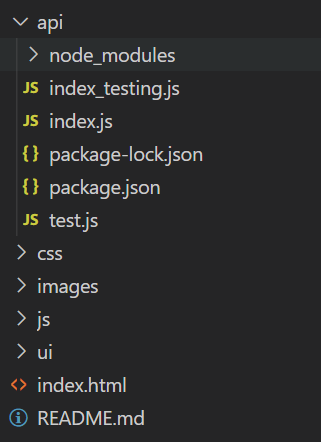
\includegraphics[scale=1]{Img/ProjectStructure.png}
    \caption{Struttura del progetto}
    \label{fig:projectStructure}
\end{figure}

\section{Project Dependencies}
I seguenti moduli Node sono stati utilizzati ed aggiunti al file \texttt{package.json}:
\begin{itemize}
    \item \texttt{Express}
    \item \texttt{Body-Parser}
    \item \texttt{Cors}
    \item \texttt{MongoDB}
    \item \texttt{Swagger-jsDoc}
    \item \texttt{Swagger-ui-Express}
    \item \texttt{sweetalert2}
\end{itemize}
\newpage
Inoltre sono stati utilizzati dei moduli per sviluppo:
\begin{itemize}
    \item \texttt{supertest}
    \item \texttt{tap-spec}
    \item \texttt{tap}
\end{itemize}

In aggiunta alle \textit{dependencies} presentate, sono stati utilizzati anche \texttt{Bootstrap}, \texttt{jQuery}, \texttt{MapBox} e \texttt{Google Charts} come script \texttt{HTML}.

\section{Project Data or DB}
Per la gestione dei dati necessari al corretto funzionamento dell'applicativo abbiamo definito 6 strutture dati come illustrato in Figura \ref{fig:DB_Structure}. Le suddette sono \texttt{"Fauna"}, \texttt{"Flora"}, \texttt{"Parco"}, \texttt{"SensoreGPS"}, \texttt{"StoricoFauna"}, \texttt{"RischioAmbientale"}.

\begin{figure}[ht]
    \centering
    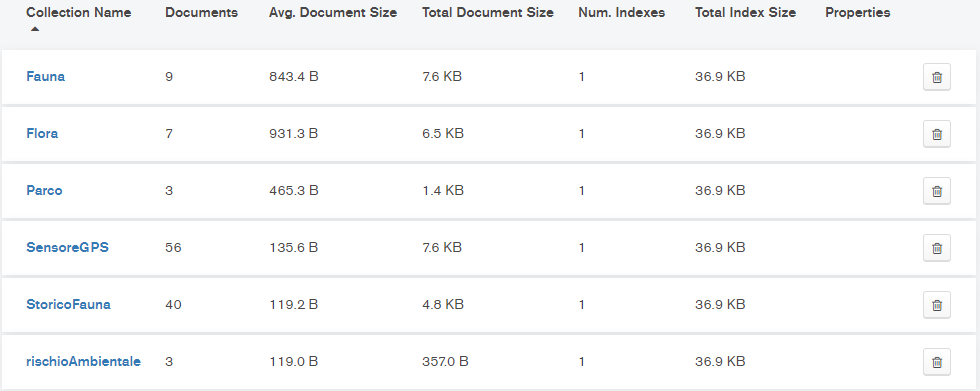
\includegraphics[scale=0.6]{Img/CollectionsMongoDB.png}
    \caption{Collezione dati utilizzati dall'applicazione}
    \label{fig:DB_Structure}
\end{figure}

\newpage
Per rappresentare le seguenti strutture dati abbiamo definito i seguenti tipi di dati (Vedi figure da \ref{fig:fauna} a \ref{fig:rischio}).

\begin{multicols}{2}
    \begin{Figure}
        \centering
        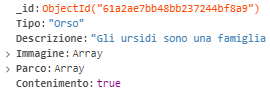
\includegraphics{Img/FaunaType.png}
        \captionof{figure}{Tipo di dato \texttt{"Fauna"}}
        \label{fig:fauna}
    \end{Figure}
    
    \begin{Figure}
        \centering
        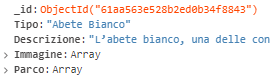
\includegraphics{Img/FloraType.png}
        \captionof{figure}{Tipo di dato \texttt{"Flora"}}
        \label{fig:flora}
    \end{Figure}
    
    \begin{Figure}
        \centering
        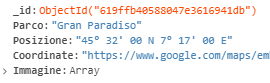
\includegraphics{Img/ParcoType.png}
        \captionof{figure}{Tipo di dato \texttt{"Parco"}}
        \label{fig:parco}
    \end{Figure}
    
    \begin{Figure}
        \centering
        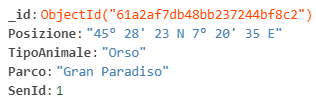
\includegraphics{Img/SensoreType.png}
        \captionof{figure}{Tipo di dato \texttt{"SensoreGPS"}}
        \label{fig:sensore}
    \end{Figure}
    
    \begin{Figure}
        \centering
        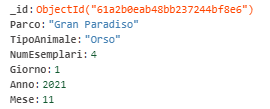
\includegraphics{Img/StoricoType.png}
        \captionof{figure}{Tipo di dato \texttt{"StoricoFauna"}}
        \label{fig:storico}
    \end{Figure}
    
    \begin{Figure}
        \centering
        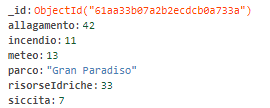
\includegraphics{Img/RischioType.png}
        \captionof{figure}{Tipo di dato \texttt{"rischioAmbientale"}}
        \label{fig:rischio}
    \end{Figure}
\end{multicols}

\newpage
\section{Project APIs}


\subsection{Elenco informazioni di un animale}
Utilizzando questa API l'applicativo può ottenere le informazioni inerenti ad un singolo animale contenuto al momento della chiamata nel sistema. L'API mediante il metodo \texttt{find(\{\})} ritorna il singolo animale inserito come parametro nella funzione. In caso venga rilevato un errore, esso verrà stampato a console.

\begin{figure}[ht]
    \centering
    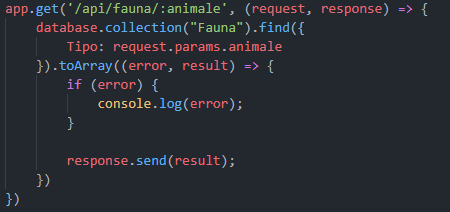
\includegraphics{Img/getFaunaByAnimal.png}
    \label{fig:get_fauna_animale}
\end{figure}

\subsection{Aggiornamento rischio ambientale in tempo reale}
La seguente API permette all'applicazione di simulare la ricezione ed inserimento nel database dei dati elaborati dal "Sistema Di Calcolo Probabilistico" (nominato molteplici volte nei documenti precedenti).

Con il metodo \texttt{updateOne(\{\},\{\})}, il sistema è in grado di modificare i valori di rischio di un parco in modo tale che le variazioni non siamo troppo elevate.

\begin{figure}[ht]
    \centering
    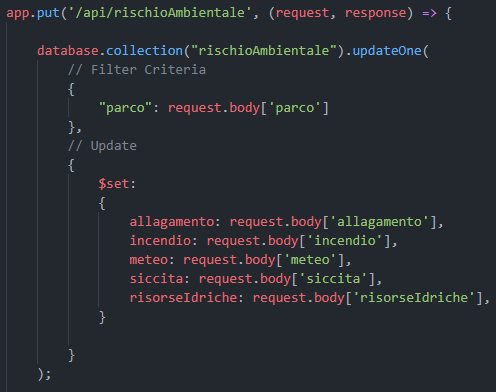
\includegraphics{Img/putRischio.png}
    \label{put_rischio}
\end{figure}

\newpage

\subsection{Aggiunta di un sensore}
Questa API viene utilizzata ogniqualvolta si desidera inserire un nuovo sensore nel sistema. 

Permette di creare un nuovo oggetto di tipo \texttt{SensoreGPS} composto da \texttt{Posizione}, \texttt{TipoAnimale}, \texttt{Parco} e \texttt{SenId} inviati come body della richiesta. Nel caso di avvenuto inserimento, viene visualizzato a console un messaggio di conferma, in caso contrario viene stampato un messaggio di errore.

\begin{figure}[ht]
    \centering
    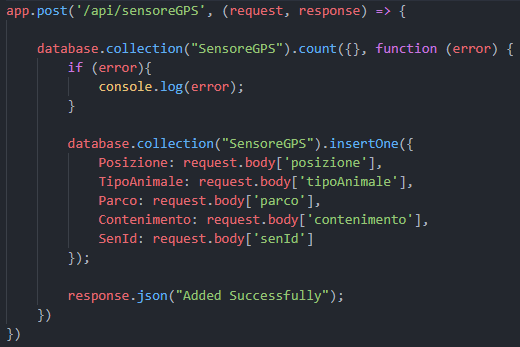
\includegraphics{Img/postSensore.png}
    \label{fig:post_sensore}
\end{figure}

\subsection{Rimozione di un sensore}
La seguente API permette all'applicazione di rimuovere un sensore dal sistema. Essa prende come input l'ID del sensore da eliminare e mediante il metodo \texttt{deleteOne(\{\})} elimina il sensore desiderato. In caso di corretta rimozione, viene visualizzato a console un messaggio di conferma.

\begin{figure}[ht]
    \centering
    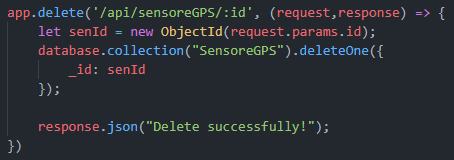
\includegraphics{Img/deleteSensore.png}
    \label{delete_sensore}
\end{figure}


% --------------- API in più -----------------

%commento
\begin{comment}
\subsection{Storico Fauna}
L'applicazione, utilizzando questa API, è in grado di ottenere dal sistema i dati relativi allo storico della fauna al momento della chiamata di quest'ultima. Essa utilizza il metodo \texttt{find({})} per ritornare i dati. Nel caso un errore venga rilevato, esso viene visualizzato a console.

\begin{figure}[ht]
    \centering
    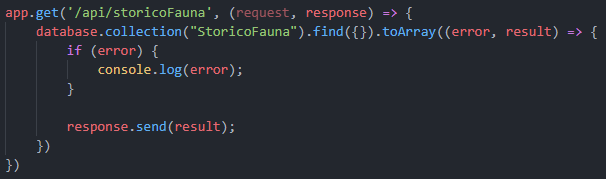
\includegraphics{Img/getStorico.png}
    \label{get_storico}
\end{figure}
\end{comment}
%commento

%commento
\begin{comment}
\subsection{Elenco fauna}
Mediante questa API l'applicazione può ottenere l'elenco degli animali contenuti al momento nel sistema. L'API ritorna l'elenco degli animali mediante il metodo \texttt{find({})} e nel caso si verifichi un errore esso verrà visualizzato a console.

\begin{figure}[ht]
    \centering
    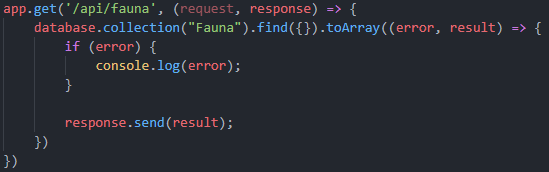
\includegraphics{Img/getFauna.png}
    \label{get_fauna}
\end{figure}
\end{comment}
%commento

%commento
\begin{comment}
\subsection{Elenco degli animali tracciati}


\begin{figure}[ht]
    \centering
    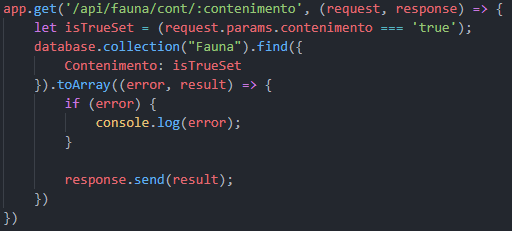
\includegraphics{Img/getFaunaByContenimento.png}
    \label{fig:get_fauna_contenimento}
\end{figure}

\subsection{Elenco flora}
Mediante questa API l'applicazione può ottenere l'elenco della fauna attualmente contenuta nel sistema. Questa API ritorna l'elenco della flora mediante il metodo \texttt{find({})} e nel caso si verifichi un errore esso verrà visualizzato a console.

\begin{figure}[ht]
    \centering
    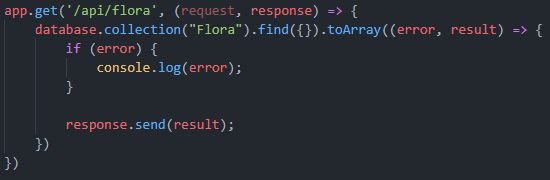
\includegraphics{Img/getFlora.png}
    \label{get_flora}
\end{figure}
\newpage
\subsection{Elenco informazioni di una pianta}

Questa API viene utilizzata dall'applicazione per ottenere i dati inerenti ad una specifica pianta. L'API ritorna la pianta selezionata utilizzando il parametro fornito in input ed utilizzandolo nel metodo \texttt{find({})}. In caso venga rilevato un errore, viene visualizzato un messaggio d'errore.
\begin{figure}[ht]
    \centering
    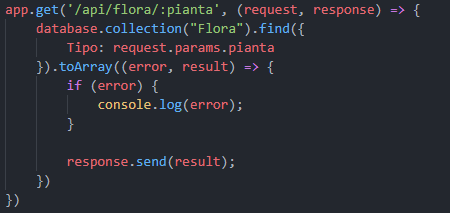
\includegraphics{Img/getFloraByPlant.png}
    \label{fig:get_flora_pianta}
\end{figure}

\subsection{Elenco parchi}
La seguente API permette all'applicazione di ottenere l'elenco dei parchi contenuti al momento all'interno del sistema ritornando il risultato del metodo \texttt{find({})}. In caso venga rilevato un errore, esso verrà stampato nella console.

\begin{figure}[ht]
    \centering
    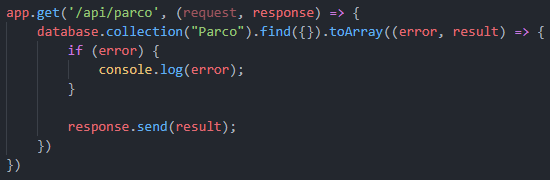
\includegraphics{Img/getParco.png}
    \label{get_parchi}
\end{figure}

\subsection{Elenco informazioni di un parco}
La seguente API permette all'applicativo di ottenere informazioni su di uno specifico parco. Essa prende in input il nome di un parco specifico ed utilizza tale argomento per selezionare, mediante il metodo \texttt{find({})}, il parco desiderato ed infine lo restituisce. In caso venga rilevato un errore, esso viene stampato in console.

\begin{figure}[ht]
    \centering
    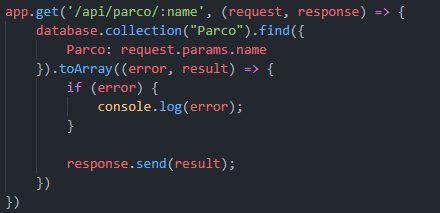
\includegraphics{Img/getParcoByName.png}
    \label{fig:get_info_parco}
\end{figure}

\newpage
\subsection{Livello Rischio}
Questa API permette all'applicazione di ottenere i livelli di rischio di tutti i parchi presenti attualmente nel sistema. L'API ritorna il risultato del metodo \texttt{find({})}, stampando a console un errore in caso esso venga rilevato.

\begin{figure}[ht]
    \centering
    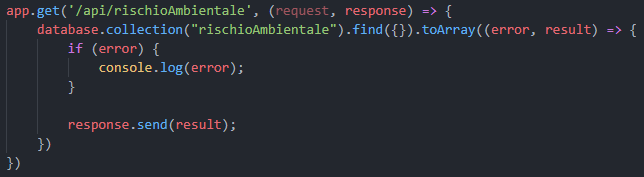
\includegraphics[scale=0.9]{Img/getRischio.png}
    \label{get_rischi}
\end{figure}

\subsection{Livello rischio di un parco}
Questa API permette all'applicazione di ottenere il livello di rischio di un parco specifico. Essa utilizza il metodo \texttt{find({})} per selezionare, utilizzando come filtro il parco inserito come argomento della funzione, i livelli di rischio del parco specifico. In caso venga rilevato un errore, esso viene visualizzato in console.

\begin{figure}[ht]
    \centering
    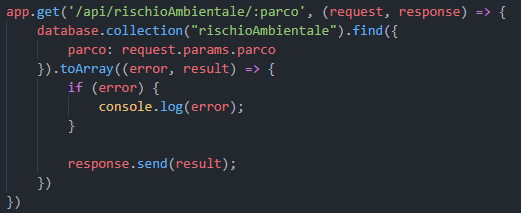
\includegraphics{Img/getRischioByParco.png}
    \label{fig:get_rischio_parco}
\end{figure}
\end{comment}
%commento

%commento
\begin{comment}
\subsection{Elenco sensori di un parco}
La seguente API permette all'applicazione di ottenere tutti i sensori GPS di un parco specifico al momento della chiamata. Ottenuto il parco come argomento della funzione, essa utilizza il metodo \texttt{find({})} per restituire tutti i sensori di quel parco specifico. In caso venga rilevato un errore, esso viene stampato a console.

\begin{figure}[ht]
    \centering
    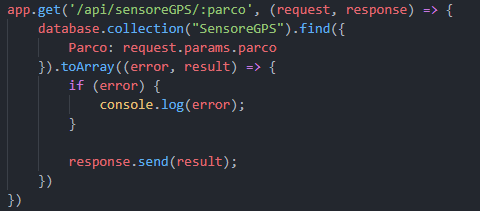
\includegraphics{Img/getSenByParco.png}
    \label{get_sensori_parco}
\end{figure}


\subsection{Elenco sensori di un animale in un parco}
La seguente API permette di ottenere i dati di uno specifico sensore in uno specifico parco presente nel sistema al momento della chiamata. Essa prende come input un animale ed un parco ed utilizzando il metodo \texttt{find({})}, seleziona il sensore correlato allo specifico animale nel parco richiesto. Un errore, in caso venga visualizzato, viene stampato in console.

\begin{figure}[ht]
    \centering
    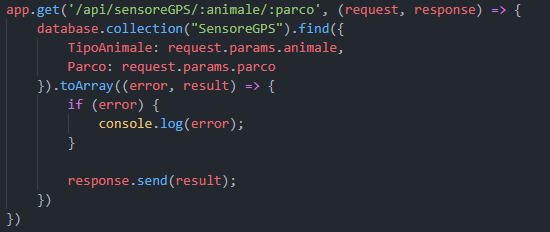
\includegraphics{Img/getSenAnimaleParco.png}
    \label{get_sensori_animale_parco}
\end{figure}
\end{comment}
%commento
\chapter{API Documentation}
Le API Locali fornite dall'applicazione Sistema Monitoraggio Ambientale e precedentemente descritte sono state documentate mediante il modulo NodeJS chiamato \texttt{Swagger-UI-Express}. Abbiamo definito le API utilizzando \texttt{JSDoc}, uno strumento volto alla generazione della documentazione utilizzando i commenti nel codice sorgente di un'applicazione. Così facendo la documentazione inerente alle API è visibile a chiunque visualizzi il codice sorgente. Per generare l'endpoint, la cui funzione è quella di presentare le API, abbiamo usato \texttt{Swagger UI} che genera una pagina web dalle definizioni delle specifiche OpenAPI.

\vspace{5mm}
\noindent
Di seguito mostriamo la pagina web contenente la documentazione che presenta le 15 API (di tipo GET, POST, PUT and DELETE) per la gestione dei dati nel nostro applicativo.

\vspace{5mm}
\noindent
La GET viene utilizzata per ottenere e visualizzare i dati in una pagina HTML. La POST serve ad inserire un nuovo dato nel sistema, la PUT modifica un dato presente nel sistema e la DELETE ne cancella uno.

\vspace{5mm}
\noindent
Dopo aver correttamente avviato le API mediante terminale, l'endpoint da invocare per poter visualizzare la seguente documentazione è: \textbf{http://localhost:49146/api-docs}

\begin{figure}[ht]
    \centering
    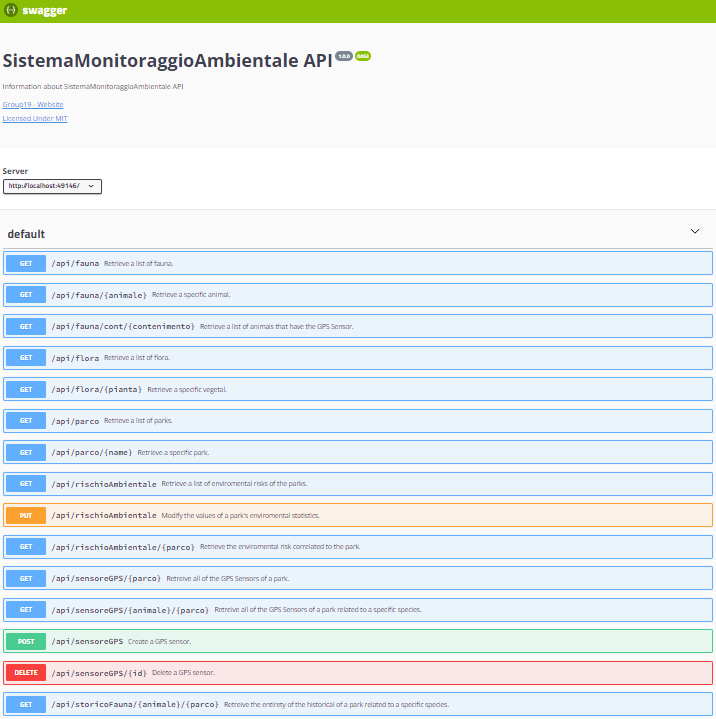
\includegraphics[scale=0.8]{Img/swagger.png}
    \caption{Documentazione delle API di Sistema di Monitoraggio Ambientale}
    \label{swagger}
\end{figure}
\chapter{Front End Implementation}

Il FrontEnd fornisce le funzionalità di visualizzazione, inserimento e cancellazione di dati dall'applicazione Sistema Monitoraggio Ambientale. L'applicazione è composta da 5 pagine: Monitoraggio, Parco, Flora, Fauna, Sensori.

\begin{figure}[ht]   
\centering
\includegraphics[scale=0.35]{Img/Menuù.png}
    \caption{Menù dell'applicazione}
    \label{Menu}
\end{figure}

Per utilizzare l'applicazione è presente un menù che guida la navigazione tra le pagine del progetto. Nelle prime tre voci, al momento della selezione si apre un menù a tendina che permette di selezionare il parco, l'animale o la vegetazione desiderata.

\begin{figure}[ht]   
\centering
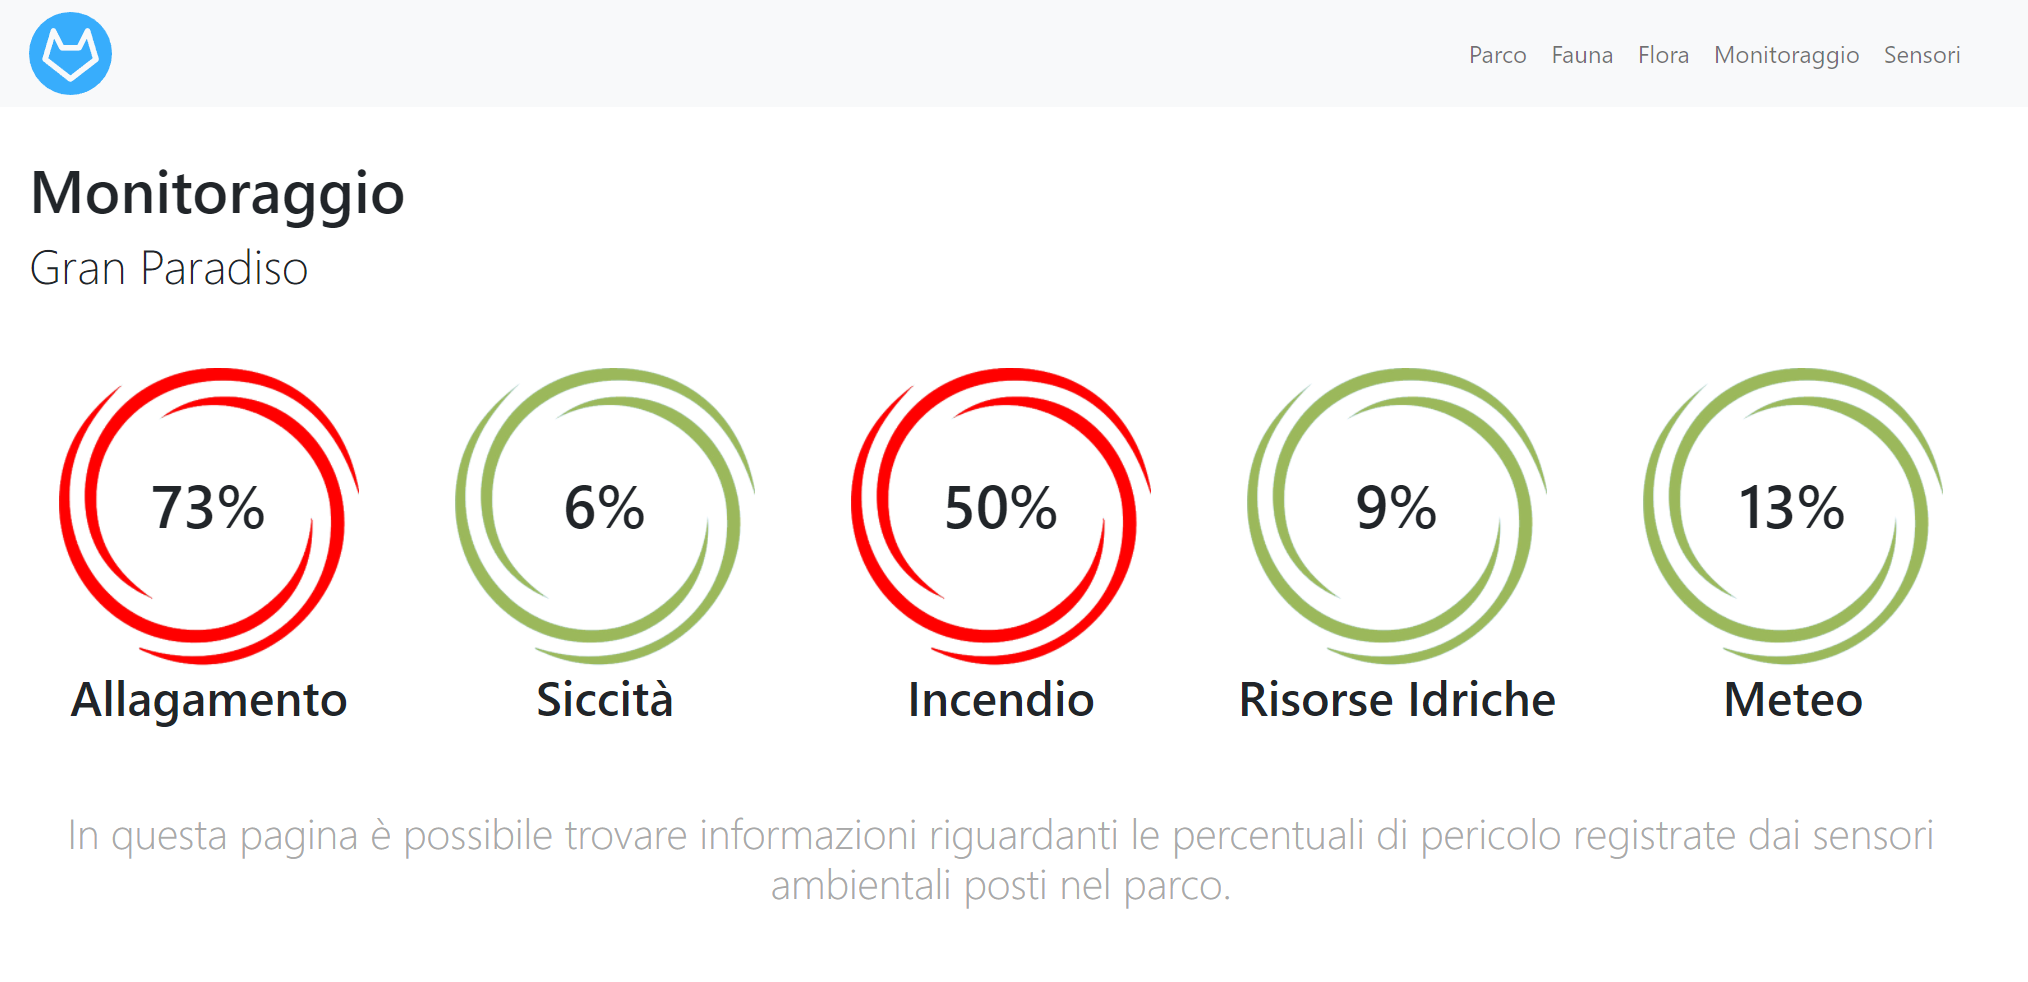
\includegraphics[scale=0.45]{Img/Monitoraggio.png}
    \caption{Pagina di Monitoraggio}
    \label{Monitoraggio}
\end{figure}


Nella Figura \ref{Monitoraggio} si possono visualizzare i livelli di pericolo delle categorie di monitoraggio del parco selezionato. In base al livello raggiunto il colore cambia tra verde, giallo e rosso.

\newpage
\begin{figure}[ht]   
\centering
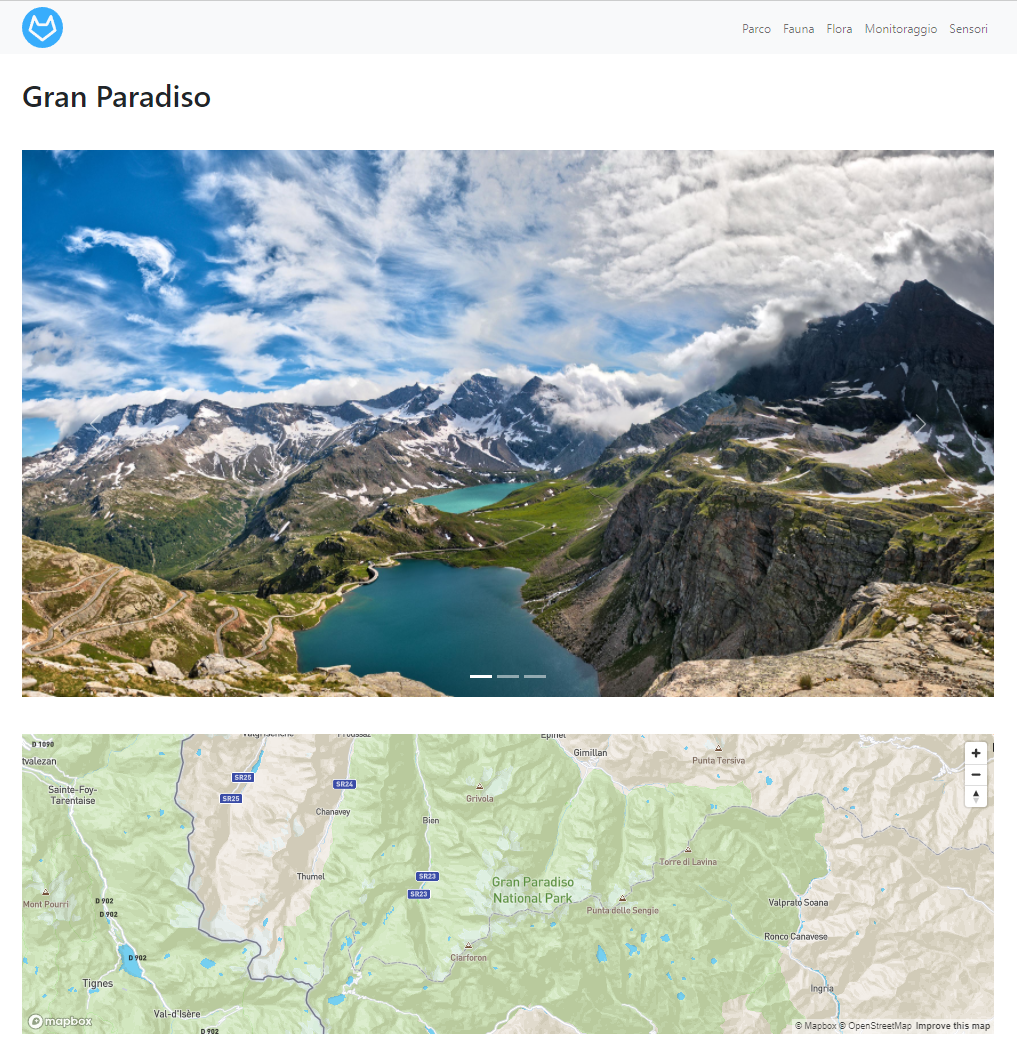
\includegraphics[scale=0.9]{Img/Parco.png}
    \caption{Esempio di Parco selezionato}
    \label{parcoselezionato}
\end{figure}

Nella Figura \ref{parcoselezionato} è possibile visualizzare delle immagini del parco ed una cartina geografica navigabile del suddetto.

\newpage

\begin{figure}[ht]   
\centering
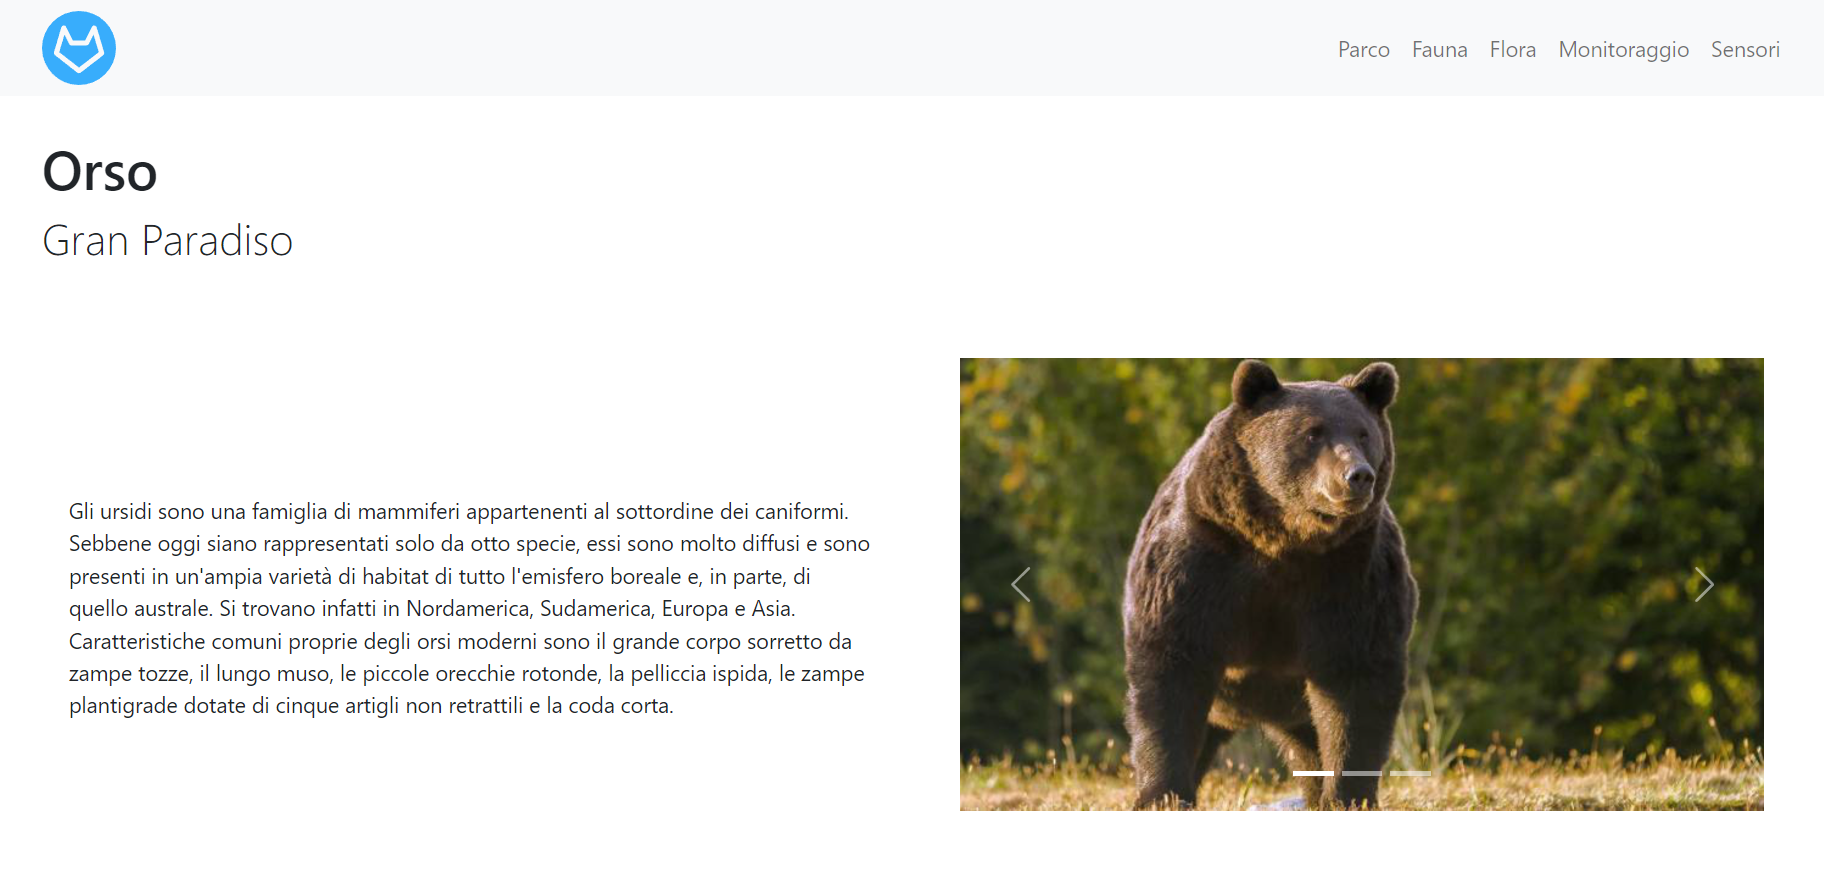
\includegraphics[scale=0.45]{Img/Fauna1.png}
    \caption{Descrizione dell'animale selezionato}
    \label{fauna1}
\end{figure}

\begin{figure}[ht]   
\centering
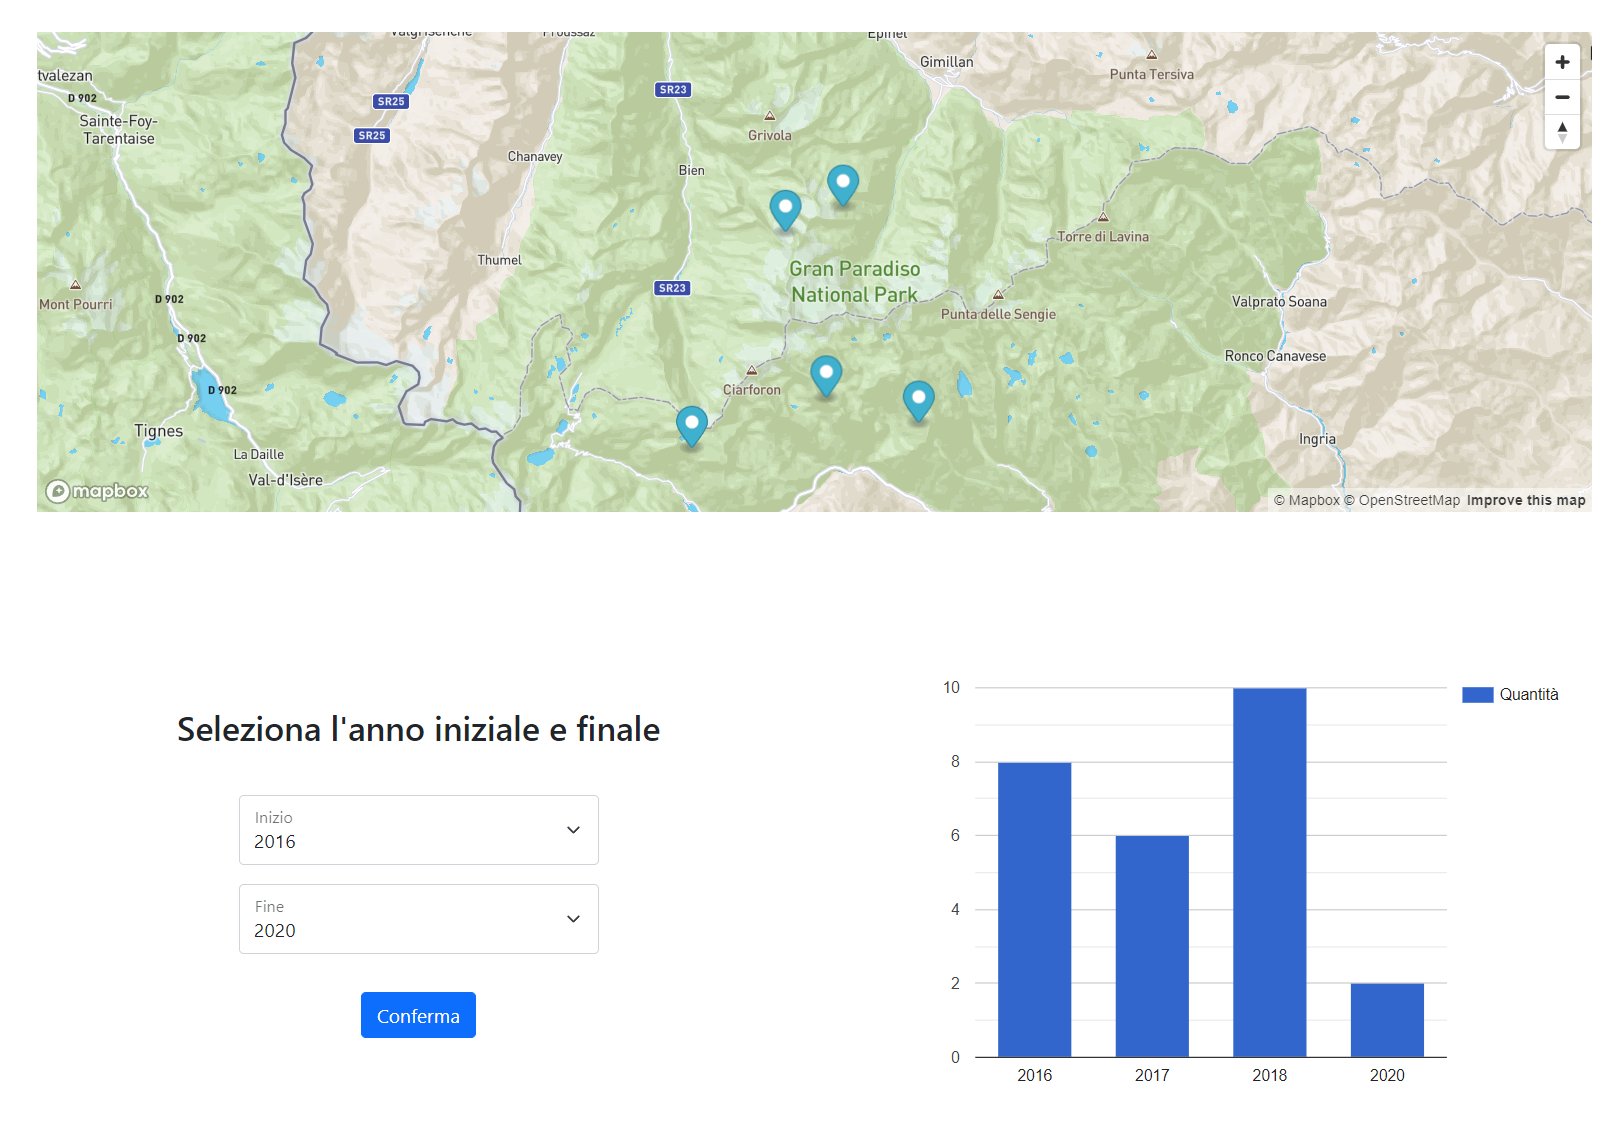
\includegraphics[scale=0.45]{Img/Fauna2.png}
    \caption{Posizione geografica e istogramma della popolazione}
    \label{fauna2}
\end{figure}

Nella figura \ref{fauna1} e \ref{fauna2} si possono visualizzare la descrizione e le immagini dell'animale selezionato. Inoltre è presente una mappa contenente dei marker che tracciano la posizione degli esemplari scelti. Infine si trova un form per inserire l'intervallo di tempo nel quale visualizzare i dati dello storico della popolazione del suddetto.

\begin{multicols}{2}
    \begin{Figure}
        \centering
        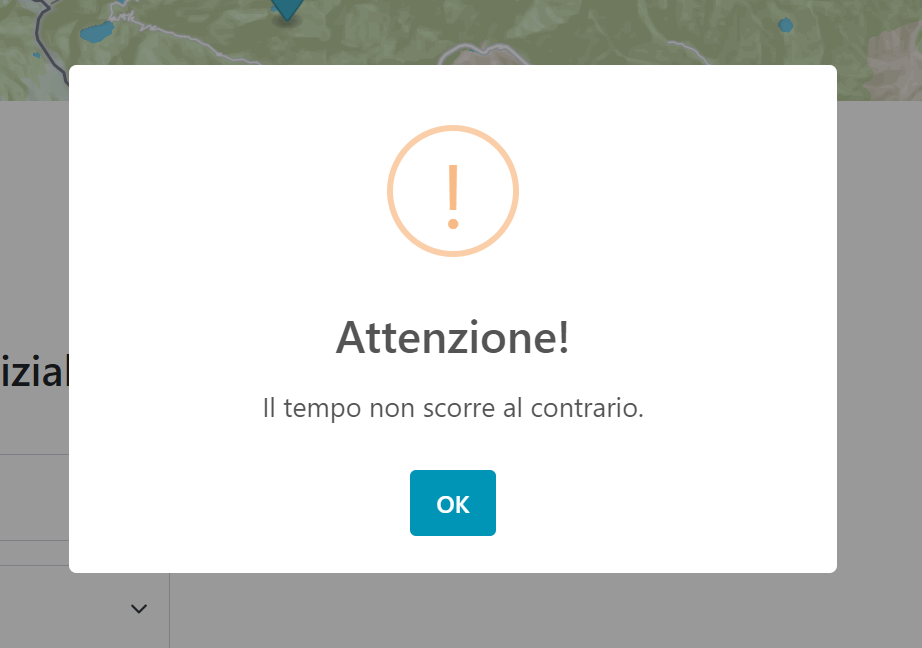
\includegraphics[scale=0.35]{Img/erroreIstogramma.png}
        \captionof{figure}{Pop-up selezione anni errati}
        \label{fig:erroreIstogramma}
    \end{Figure}
    \columnbreak
    Nel caso in cui l'utente selezioni una data di inizio maggiore a quella di fine viene mostrato un pop-up di avvertimento \ref{fig:erroreIstogramma}.
\end{multicols}

\newpage
\begin{figure}[ht]   
\centering
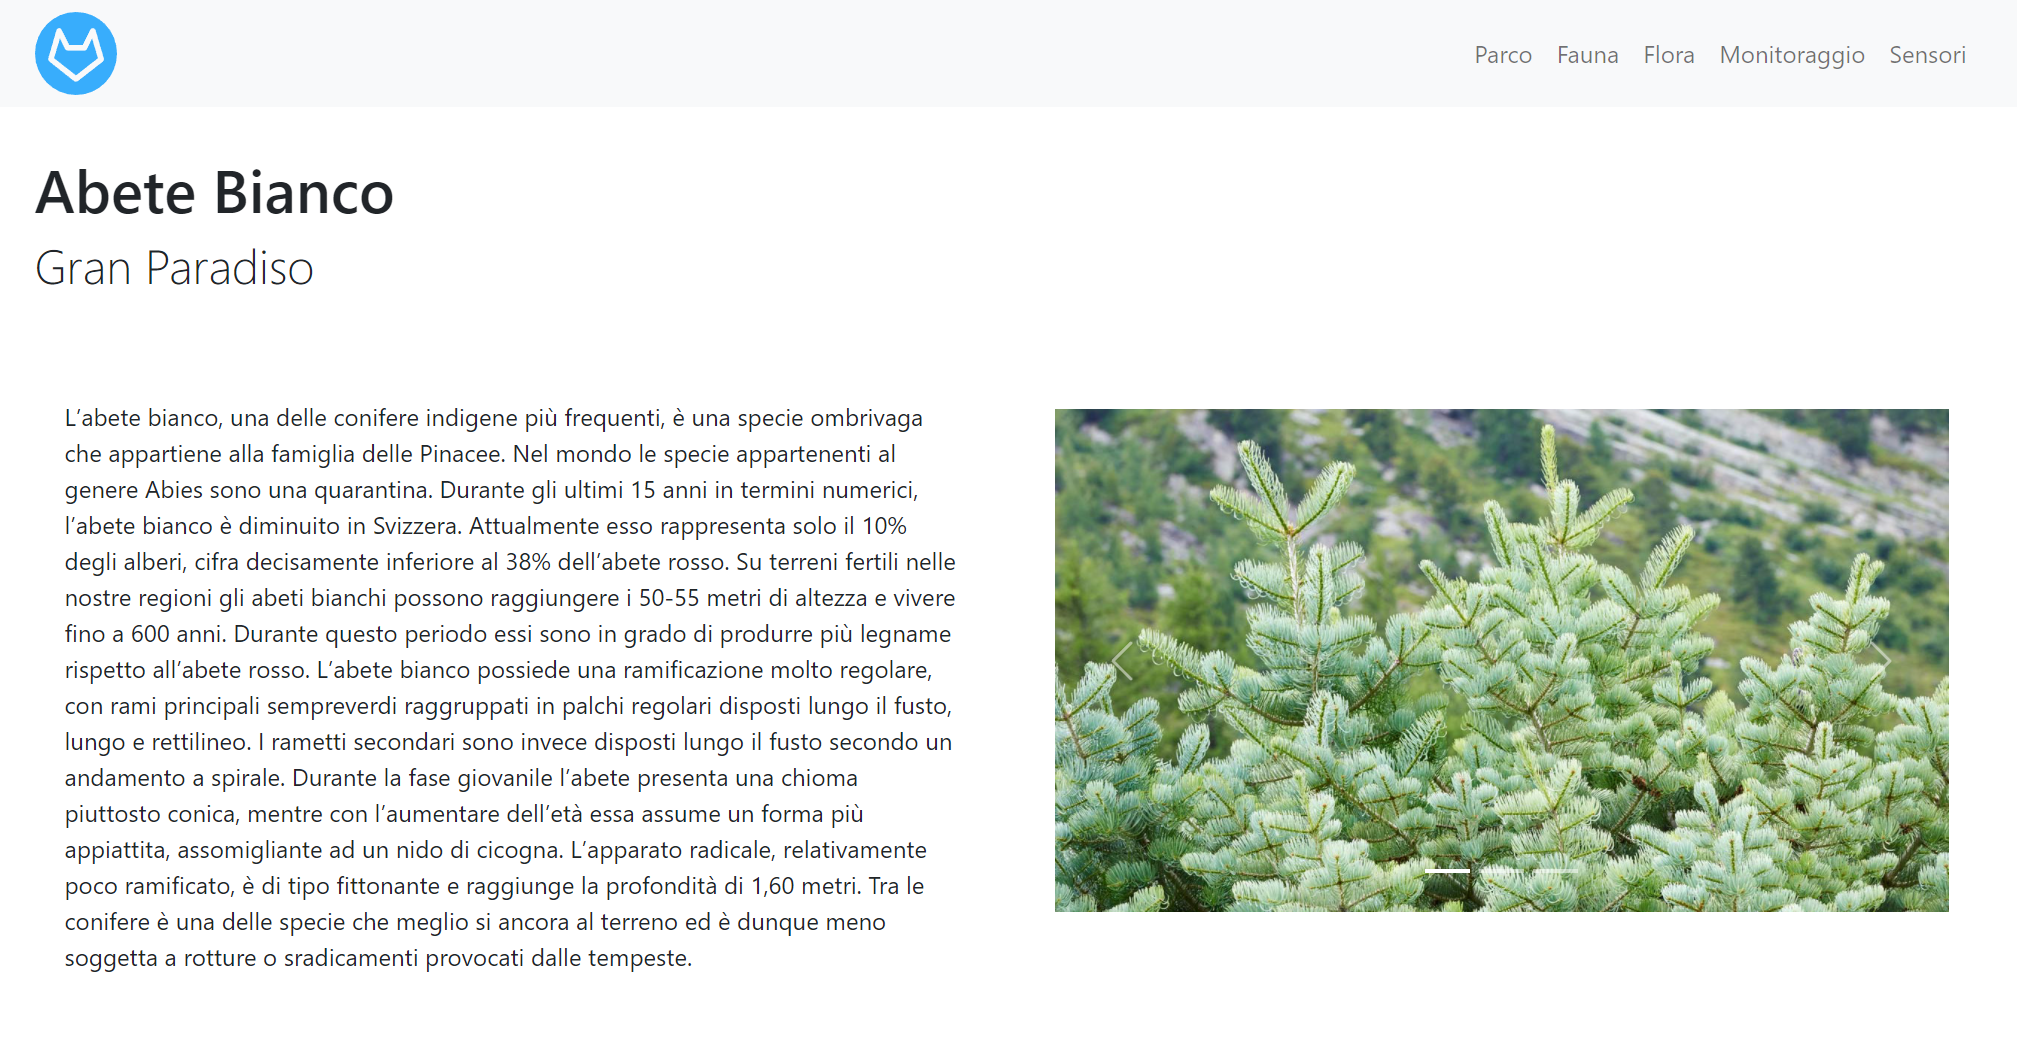
\includegraphics[scale=0.45]{Img/Flora.png}
    \caption{Pagina Flora dell'applicazione Sistema Monitoraggio Ambientale}
    \label{flora}
\end{figure}

Nella figura \ref{flora} si possono visualizzare descrizione ed immagini della specie vegetale selezionata.

\begin{figure}[ht]   
\centering
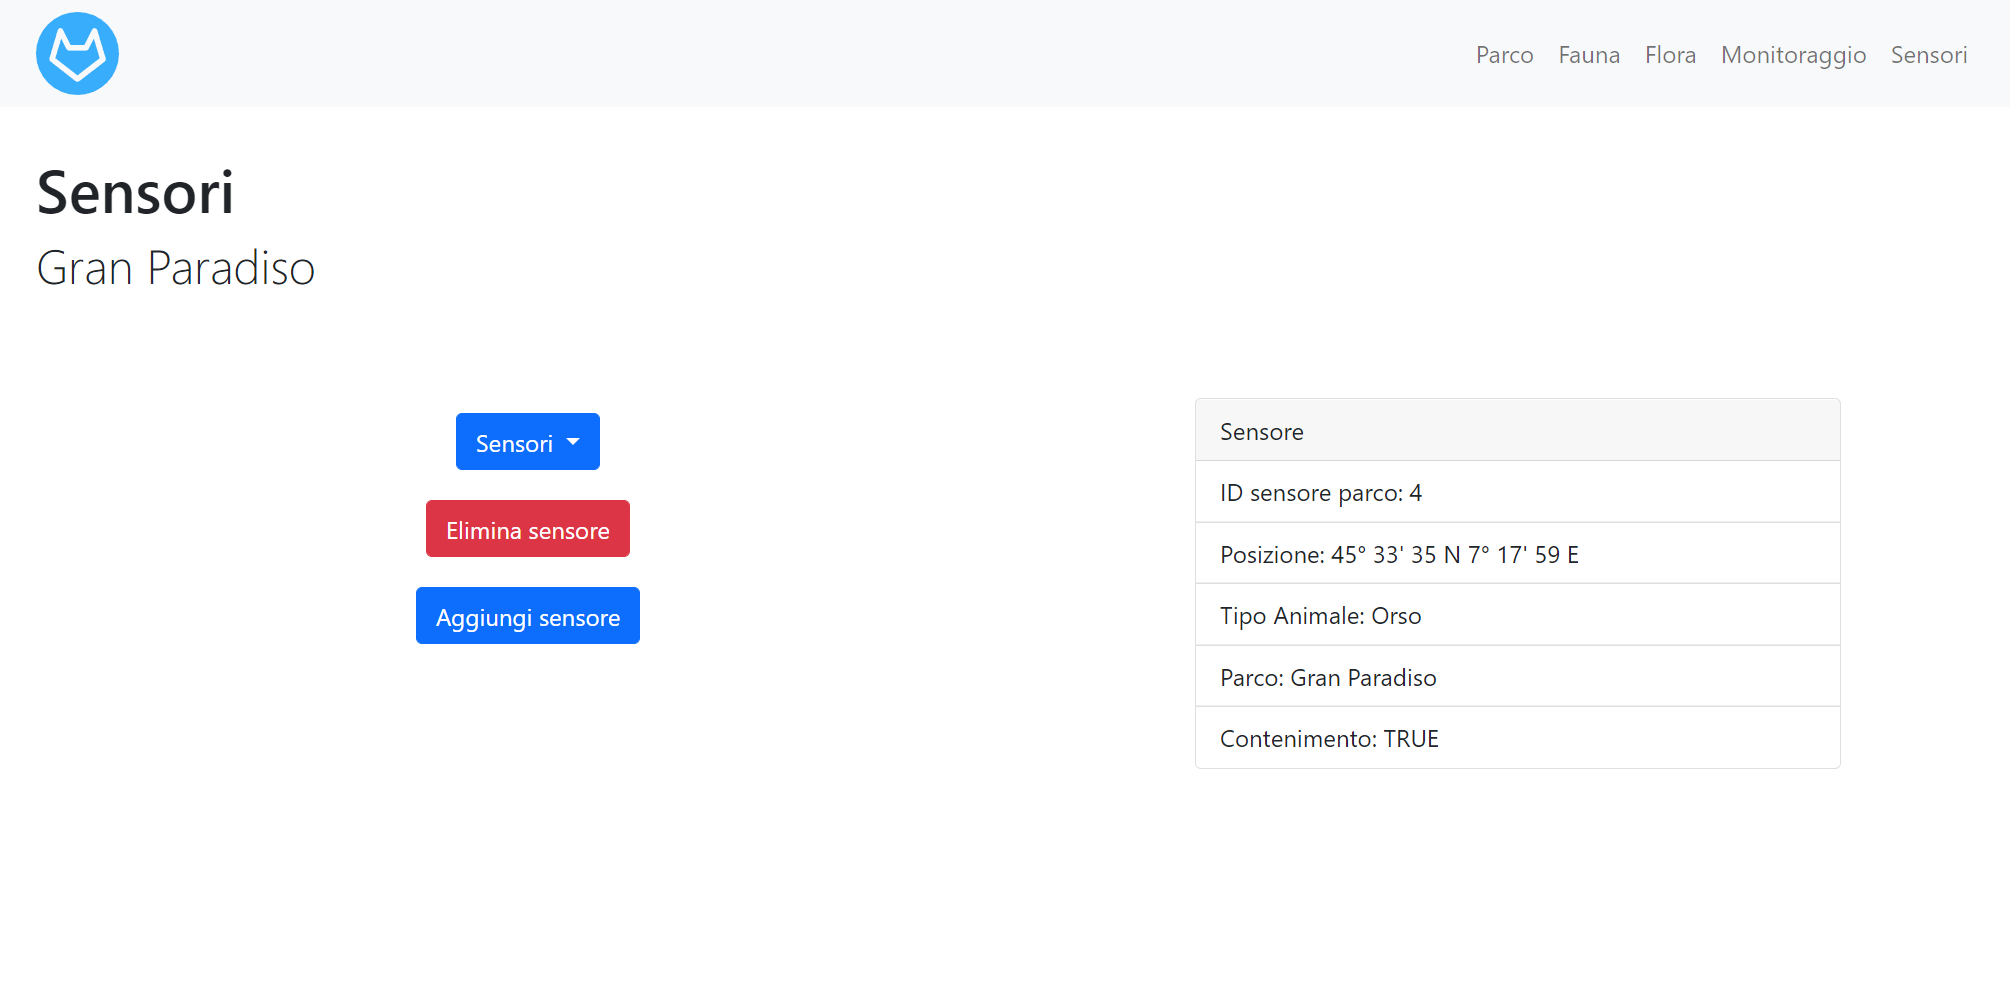
\includegraphics[scale=0.45]{Img/Sensori.png}
    \caption{Pagina dei Sensori}
    \label{sensorilista}
\end{figure}

Nella figura \ref{sensorilista} troviamo nella parte sinistra la possibilità di selezionare, eliminare
ed aggiungere un sensore, mentre nella parte destra una tabella sulla qualche visualizzare i dati del sensore selezionato.
\noindent
L'opzione "Elimina sensore" viene resa disponibile dopo aver selezionato un sensore e permette di eliminare quel preciso sensore dalla lista, notificando l'utente mediante un pop-up.

\newpage
\begin{multicols}{2}
    \begin{Figure}
        \centering
        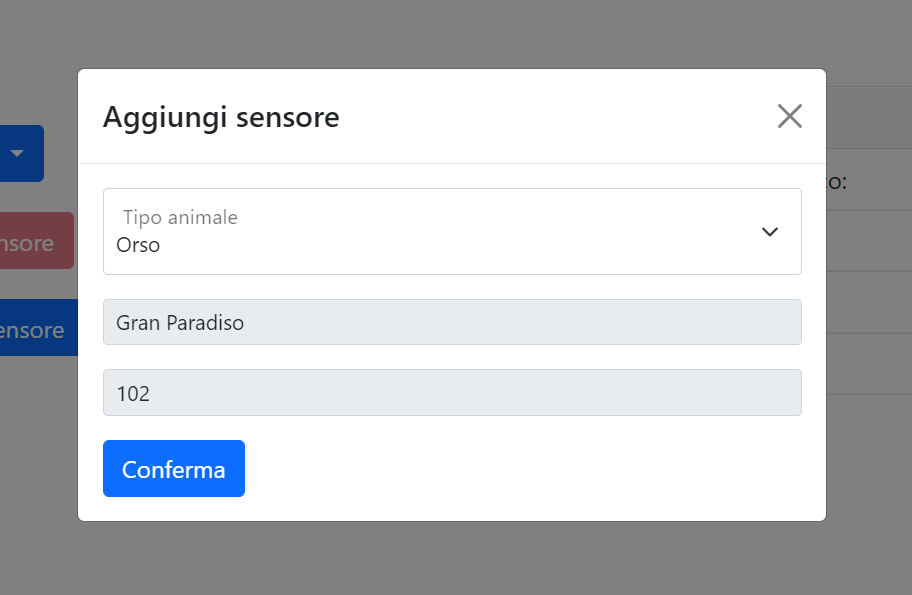
\includegraphics[scale=0.5]{Img/aggiungiSensore.png}
        \captionof{figure}{Form aggiungi sensore}
        \label{fig:formAggiungiSensore}
    \end{Figure}
    \begin{Figure}
        \centering
        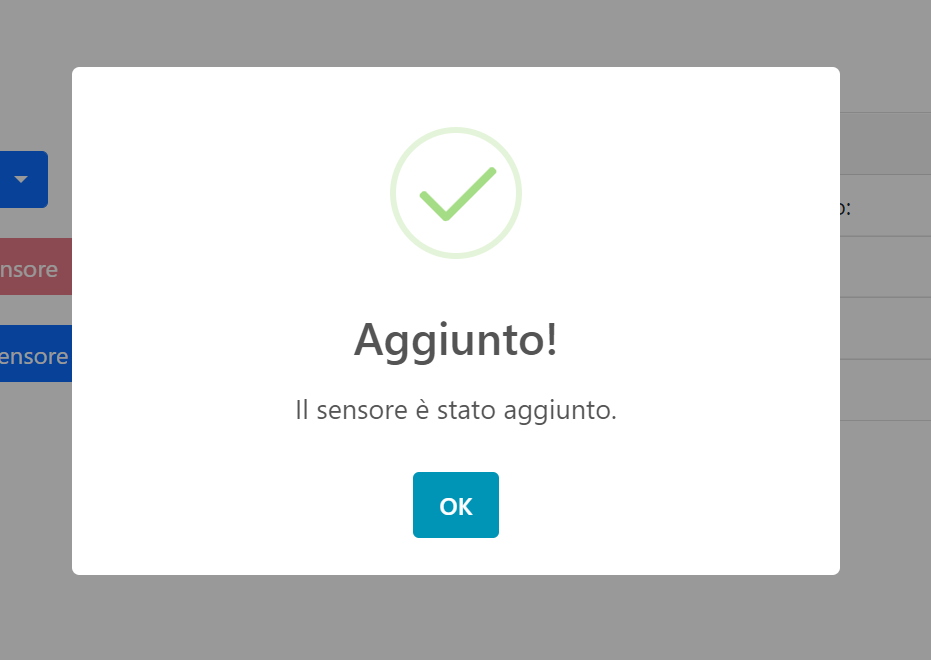
\includegraphics[scale=0.45]{Img/avvenutaAggiunta.png}
        \captionof{figure}{Pop-up conferma}
        \label{fig:avvenutaAggiunta}
    \end{Figure}
\end{multicols}

Nel caso in cui si volesse aggiungere un sensore (figura \ref{fig:formAggiungiSensore}), l'amministratore deve inserire il tipo di animale, mentre 
i campi "Parco" e "ID sensore parco" sono precompilati dal programma, il quale assegna tali valori in base al parco e al numero di sensori presenti in esso nel momento dell'inserimento.

Come definito dallo User Flow al capitolo \ref{capitolo3}, il sistema prevede l'invio di conferma aggiunta sensore (figura \ref{fig:avvenutaAggiunta}) come anche un pop-up che richieda se l'utente è sicuro di voler eliminare un sensore (figura \ref{fig:richiestaEliminazine}) e di seguito l'avvenuta eliminazione (figura \ref{fig:avvenutaEliminazione}).

\begin{multicols}{2}
     \begin{Figure}
        \centering
        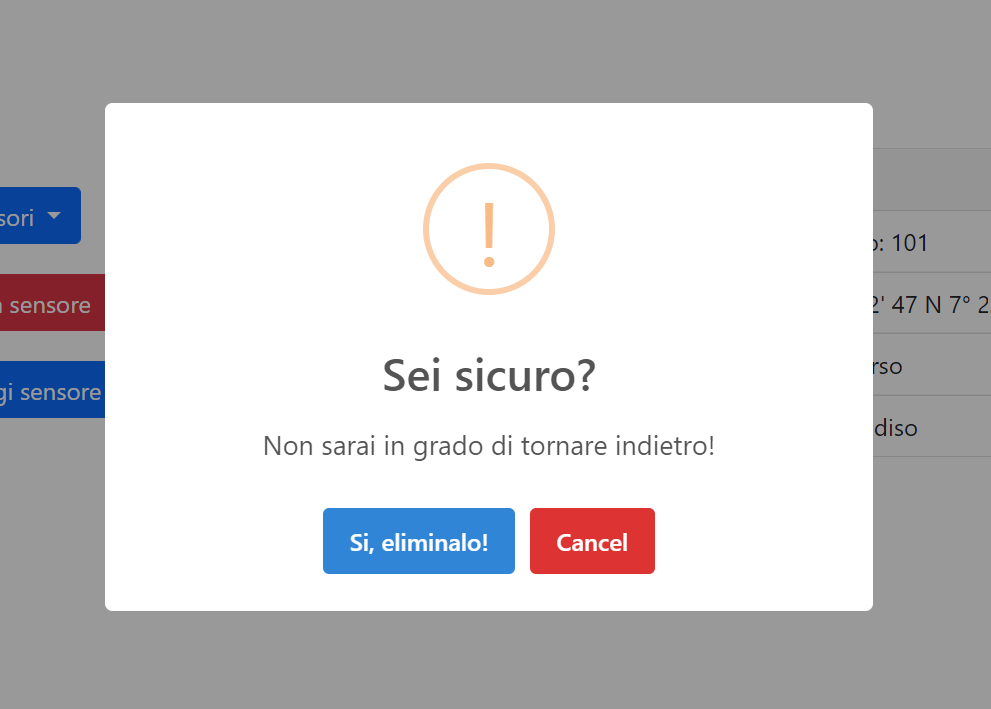
\includegraphics[scale=0.45]{Img/confermaEliminazione.png}
        \captionof{figure}{Form aggiungi sensore}
        \label{fig:richiestaEliminazine}
    \end{Figure}
    \begin{Figure}
        \centering
        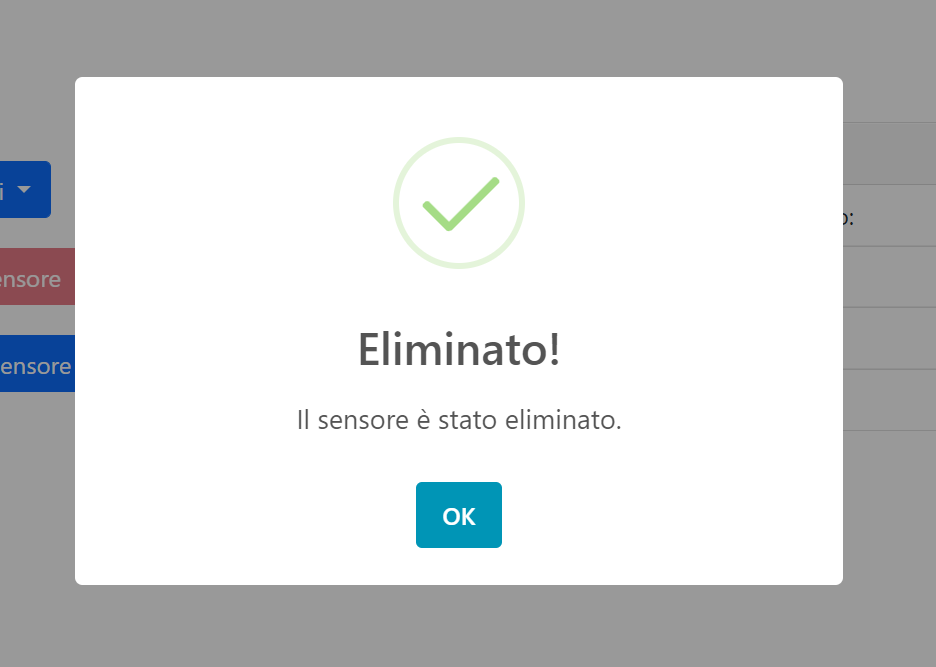
\includegraphics[scale=0.47]{Img/eliminato.png}
        \captionof{figure}{Pop-up conferma}
        \label{fig:avvenutaEliminazione}
    \end{Figure}
\end{multicols}


\chapter{GitHub Repository Info}

Il progetto Sistema di Monitoraggio Ambientale è disponibile al seguente link: \textbf{\textcolor{black}{\href{https://github.com/luiss07/SistemaMonitoraggioAmbientale}{Sistema di Monitoraggio Ambientale repository}}}. Per poter eseguire il progetto è sufficiente avviare il server mediante il comando \textbf{npm start} all'interno della cartella \texttt{api}. Per quanto riguarda il client, invece, è sufficiente aprire il file \texttt{index.html} contenuto nella cartella principale utilizzando un live server (consigliato quello di vscode).
\chapter{Testing}
Per effettuare il testing abbiamo definito all'interno della cartella \texttt{api} uno script \texttt{test.js} che contiene i test delle quattro tipologie di api e uno script \texttt{index\_testing.js} dove sono definite le api su cui viene eseguito. L'obiettivo di questo testing è quello di verificare la corretta esecuzione delle api \texttt{GET}, \texttt{POST}, \texttt{DELETE} e \texttt{PUT}.

\vspace{5mm}
Per eseguire il test abbiamo esteso il file di configurazione \texttt{package.json} con la seguente riga di codice \texttt{"text" = "node test | tap-spec"}.

\begin{figure}[ht]
    \centering
    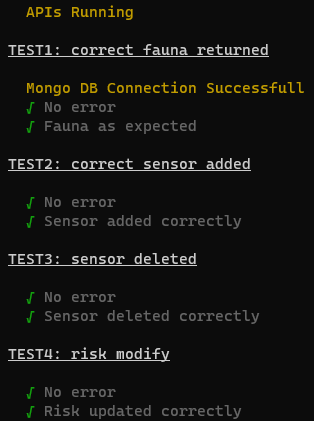
\includegraphics[scale=0.7]{Img/testing_result.png}
    \caption{Esito del testing}
\end{figure}

\end{document}
